\chapter{Peierls-Hubbard model}
\label{chap:model}

As mentioned in section \ref{sec:overview}, treatments based in the adiabatic and antiadiabatic approximations are unable to describe properly the correlated charge-ion motion in cuprate's Cu-O bonds.
An alternative to overcome this limitation is an exact treatment of a reduced system.
In this thesis we focus on the O(4)-Cu(1)-O(4) cluster in YBa$_2$Cu$_3$O$_7$.
We approximate this local environment as a three site cluster with two holes. 
Such approximation is justified as the Cu(1)-O(4) bond length (1.83 \AA) is far shorter than the Cu(2)-O(4) bond length ($\sim 2.41$ \AA) (see figure \ref{fig:YBCO_structure}), making charge transfer outside the cluster a much slower process than the charge dynamics inside the cluster. 
Although we cannot directly identify the three site cluster proposed in this model with a particular structure of the CuO plane, the general approach of charge transfer between hole rich regions and hole poor regions in the plane coupled to the lattice degrees of freedom is still valid, hence the general conclusions we draw from this model are applicable to describe the structure of the CuO plane.

This thesis is based in a thorough analysis of that model hamiltonian so we devote this chapter to a detailed description of its components.
In section \ref{sec:hamiltonian-and-basis} we describe the hamitlonian and the basis used. 
Section \ref{sec:isotopic-model} reviews a method of incorporating isotopic substitutions in this model and defines \textit{isotopic shifts} in this context.
In section \ref{sec:lattice-distortions} we discuss a method of calculating real-space lattice distortions.
Next, in section \ref{sec:chargeLocalization}, we describe a projection into definite charge occupation states.
Section \ref{sec:model-parameters} reviews some literature suggesting possible choices of parameters and lists the parameters used in this work.
We review in section \ref{sec:classification} a method for identifying and classifiying the different excitations in this model.
Computational details about the calculations can be found online\footnote{https://research-engine.appspot.com/37001/notebooks/2001}.

\section{Hamiltonian and basis set}
\label{sec:hamiltonian-and-basis}

To describe two holes in the O(4)-Cu(1)-O(4) cluster with an charge-ion (phonon) correlated movement we use a hamiltonian consisting of three parts:
%
\begin{equation}
  \label{eq:full-hamiltonian}
  H = H_{el} + H_{ph} + H_{el-ph}
\end{equation}
%
corresponding to the electronic contribution, the phonon energies and the electron-phonon (lattice) coupling, respectively \cite{Salkola1994}. 
The electron-phonon coupling term deviates this model from the Born-Oppenheimer (adiabatic) approximation and prevents the separation of hamiltionan eigenstates, $\Psi$, as products of purely electronic and phononic parts, $\Psi=\psi_{el}\psi_{ph}$, unless $H_{el-ph}=0$.
Nonetheless, as it will be discussed in section \ref{sec:classification}, even for coupling values greater than zero the hamiltonian eigenstates can be interpreted as mainly \textit{electronic} or \textit{phononic} in nature.

The electronic part is modeled as a single band Hubbard model for three sites with two holes in it. 
We only consider the two holes as having opposite spin because the energies of states with two charges with the same spin are much greater.
Explicitly, $H_{el}$ is written as
%
\begin{equation}
  \label{eq:electronic-part}
  H_{el} = \sum_{\sigma,i=1}^3 E_i n_{\sigma i} 
        + U\sum_{i=1}^3 n_{i\downarrow}n_{i\uparrow} 
        + t\sum_{\sigma} \left(c_{1\sigma}^\dagger c_{2\sigma} + c_{2\sigma}^\dagger c_{3\sigma} + H.c. \right)
\end{equation}
%
where we denoted $n_{i\sigma}=c_{i\sigma}^\dagger c_{i\sigma}$ as the hole-number operator with $c_{i\sigma}^\dagger$ creating a hole with spin $\sigma = \uparrow, \downarrow$ and $c_{i\sigma}$ destroying it; the site index $i=1,2,3$ indicates the two oxygen sites [O(4)] when  $i=1,3$ and the only copper site [Cu(1)] when $i=2$. 
The site energies are parametrized with $E_1=E_3=-E_2 \equiv E_0$.\footnote{In \cite{Salkola1995} the authors consider an example of \textit{disorder} in this system by letting $E_1\neq E_3$.}
$U$ is the on-site Coulomb interaction and $t$ is the hopping energy between two adjacent sites. 

For the lattice  part of the Hamiltonian, $H_{ph}$, we consider both symmetric (Raman) and antisymmetric (infrared) modes described by boson operators $b_R$ and $b_{ir}$ and bare frequencies $\omega_R$ and $\omega_{ir}$ respectively,\footnote{Unlike previous publications, here we include the \textit{zero-point energy} for both phonon modes. 
For most cases this is not needed since the excitation's energies are calculated relative to the ground state but, in chapter \ref{chap:ground} we study the ground state energy itself where this contribution is important.}
%
\begin{equation}
 \label{eq:phonon-part}
 H_{ph} = \hbar \omega_{ir}\left(b_{ir}^\dagger b_{ir}+\frac{1}{2}\right) + \hbar \omega_R \left( b_R^\dagger b_R + \frac{1}{2}\right)
\end{equation}
%
\begin{figure}[ht]
  \centering
  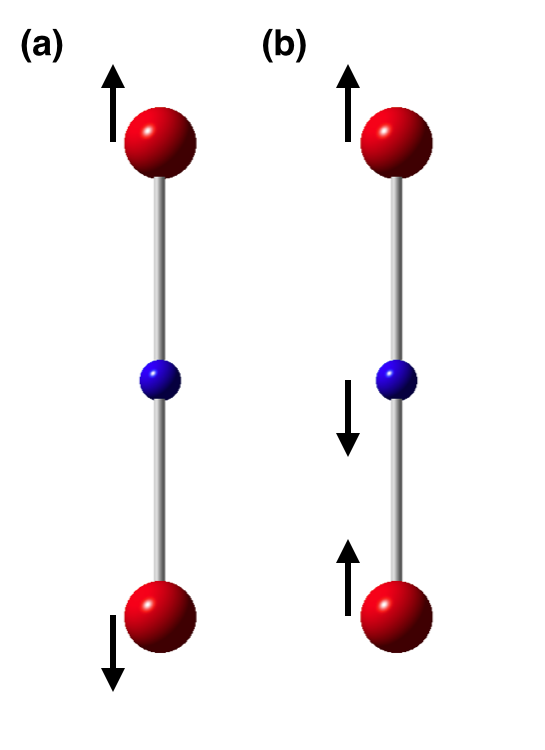
\includegraphics[width=0.3\textwidth]{images/CuO2-vibrations.png}
  \caption[Schematic for the symmetric (Raman) and antisymmetric (infrared) vibrational modes in CuO$_2$.]
  {Schematic showing the \textbf{(a)} symmetric (Raman) and \textbf{(b)} antisymmetric (infrared) vibrational modes for the CuO$_2$ cluster.}
  \label{fig:CO2-vibrations}
\end{figure}

The electron-lattice coupling term, $H_{el-ph}$ is introduced through the change in interatomic distances generated by Coulomb repulsion between different sites coupled with the Raman and infrared phonon modes,
%
\begin{equation}
  \label{eq:prev-coupling-part}
  H_{el-ph} = \tilde{\lambda_{ir}}u_{ir}(n_3 - n_1) + \tilde{\lambda_R} u_R (n_1 + n_3-s_0)
\end{equation}
%
Here $u_{ir}$ and $u_R$ are the \textit{phonon coordinates} for the infrared and Raman modes respectively, they are related to the atomic coordinates $x_i=1,2,3$ by
%
%
\begin{equation}
  \label{eq:uR}
  u_R \equiv \left(\frac{\hbar}{2 m_R \omega_R}\right)^{1/2}(b_R^\dagger + b_R) = \frac{x_3 - x_1}{\sqrt{2}}
\end{equation}
%
\begin{equation}
  \label{eq:uir}
  u_{ir} \equiv \left(\frac{\hbar}{2 m_{ir} \omega_{ir}}\right)^{1/2}(b^\dagger_{ir}+b_{ir}) = \frac{ x_1 + x_3 - ( 2 m_O/m_{Cu})x_2}{(2 + 4 m_O/m_{Cu})^{1/2}}
\end{equation}
%
with $m_{ir}$ and $m_R$ being the reduced mass for each mode (see (\ref{eq:redMassR}, \ref{eq:redMassIr}) below), $x_i=2$ the position of the central copper atom and $x_i=1,3$ the positions of the oxygen atoms.
The constant $s_0$ is introduced to avoid artificial shrinking of the cluster\footnote{This term is written slightly different in some publications, for example in \cite{MustredeLeon1992}, $H_{el-ph}$ is proportional to $n_1-n_2+n_3$. However both versions can be related noticing that $3 (n_1+n_3-4/3)=n_1-2n_2+n_3$.}. 
For consistency with other works \cite{MustredeLeon1992,DeLeon1999,Leon2008,MirandaMena2007} we fix $s_0=4/3$. 
Using the definitions (\ref{eq:uR}, \ref{eq:uir}) we can rewrite (\ref{eq:prev-coupling-part}) as
%
\begin{equation}
  \label{eq:coupling-part}
  H_{el-ph} = \lambda_{ir}(b_{ir} + b_{ir}^\dagger)(n_3 - n_1) + \lambda_R (b_R + b_R^\dagger) (n_1 + n_3-s_0)
\end{equation}
%
With 
%
\begin{equation}
  \label{eq:coupling-constants}
  \lambda_R=\tilde{\lambda_R}(\hbar/2m_R\omega_R)^{1/2},\ \ \lambda_{ir}=\tilde{\lambda_{ir}}(\hbar/2m_{ir}\omega_{ir})^{1/2}
\end{equation}
From the definition of $H_{el-ph}$ we can observe that the electrons will be coupled to the infrared (antisymmetric) mode only when one charge is located at the copper site and the other in an oxygen.
However, there will be electron-lattice coupling with the Raman (symmetric) mode in all cases.

One simple basis set for this system can be denoted as $\{\ket{e_1,e_2,ir,R}: e_1,e_2=1,2,3; ir,R=1,2,\ldots\}$ with $e_k$ being the position of the $k$-th hole, $ir$ the number of \textit{infrared} phonons and $R$ the number of \textit{Raman} phonons. 
This basis is infinite dimensional however for the lower energy excitations the eigenvalues and eigenvectors are well described using a basis with only a few phononic excitations.

\section{Lattice distortions}
\label{sec:lattice-distortions}

With the atomic coordinates $x_i$ as defined before ($i=1,3$ for the oxygens and $i=2$ for the copper) the distance difference $d$ between one O-Cu bond and the other is
%
\begin{equation}
  \label{eq:bondDiff}
  d =  (x_3 - x_2) - (x_2 - x_1) = x_1 + x_3 - 2x_2 
\end{equation}
%
The $x_i$ coordinates are varying at all times but taking an instant in which $x_2=0$ we can simplify (\ref{eq:bondDiff}) to
%
\begin{equation}
  \label{eq:bondDiffSimpl}
  d = x_1+x_3
\end{equation}
%
Which can be related to the phonon coordinate $u_{ir}$ by using (\ref{eq:uir}) with $x_2=0$,
%
\begin{equation}
  \label{eq:uirSimpl}
  u_{ir}=\frac{x_1+x_3}{\left( 2+4 m_O/m_{Cu} \right)^{1/2}}
\end{equation}
%
Substitution (\ref{eq:bondDiffSimpl}) into (\ref{eq:uirSimpl}) and solving for $d$ gives
%
\begin{equation}
  \label{eq:dvsuir}
  d=\sqrt{2}\left(1 + 2\frac{m_O}{m_{Cu}} \right)^{1/2}u_{ir}
\end{equation}
%
which is a relationship between the phonon coordinates, that can be calculated from the model's eigenfunctions, and the observable lattice distortion.
Equation (\ref{eq:dvsuir}) allows a conection between this model hamiltonian and a specific experimental observation. 
It is this relationship that helps fixing the free coupling parameters $\lambda_{ir}$ and $\lambda_R$ in this model.

In the remainder of this section we show how to find the most probable $u_{ir}$ value for a given state in the model hamiltonian (\ref{eq:full-hamiltonian}).
To do this we first take as an example a simple quantum harmonic oscillator 
%
\begin{equation}
  \label{eq:harmOscHam}
  H=\hbar\omega \left(a^\dagger a + \frac{1}{2}\right)
\end{equation}
with mass $m$ and frequency $\omega$.
The creation ($a^\dagger$) and annihilation ($a$) operators are related to the real-space position coordinate $u$ as
%
\begin{equation}
  \label{eq:harmOscRel}
  u=\sqrt{\frac{\hbar}{2m\omega}}\left(a+a^\dagger\right)
\end{equation}

An energy eigenfunction, $\ket{n}$ where $n$ labels the \textit{number of phonons}, has a projection into the real space coordinate $u$ given in terms of a Hermite polynomial $H_n(u)$ of degree $n$ in the following way,
%
\begin{equation}
  \label{eq:harmOscProj}
  \braket{u}{n} 
  \equiv \psi_n(u) 
  = \frac{1}{\sqrt{2^n n!}} \left(\frac{m \omega}{\pi \hbar}\right)^{1/4}
  \exp\left(-\frac{m \omega u^2}{2 \hbar}\right) H_n\left( \sqrt{\frac{m \omega}{\hbar}} u \right) 
\end{equation}
%
An arbitrary wavefunction $\ket{\psi}$ can be expanded in terms of the energy eigenfuntions as $\ket{\psi} = \sum_n \braket{n}{\psi} \ket{n}$ and projected in real space: $\braket{u}{\psi} = \sum_n \braket{n}{\psi} \braket{u}{n}$ with $\braket{u}{n}$ given by (\ref{eq:harmOscProj}).

Now, returning to the model hamiltonian (\ref{eq:full-hamiltonian}), as discussed in section \ref{sec:hamiltonian-and-basis}, a possible basis set is given by the functions ${| e_1, e_2, ir, R \rangle}$ with $e_i$ the position of the $i$-th electron and $ir$, $R$ the number of infrared and Raman phonons respectively. 
Thus an arbitrary wavefunction in this system, $\ket{\psi}$, can be expanded in this basis as
%
\begin{equation}
  \label{eq:wf-phonon-base}
  \ket{\psi}=\sum_{e_1,e_2,ir,R} \braket{e_1,e_2,ir,R}{\psi}\ket{e_1,e_2,ir,R}
\end{equation}
%
and we can make the partial projection into the phonon coordinates $(u_{ir},u_R)$ as defined by (\ref{eq:uR},\ref{eq:uir}) in the following way
%
\begin{equation}
  \label{eq:wf-expansion}
  \braket{u_{ir},u_R}{\psi}=\sum_{e_1,e_2,ir,R} \braket{e_1,e_2,ir,R}{\psi}\braket{u_{ir},u_R}{ir,R}\ket{e_1,e_2}
\end{equation}
%
where we have denoted $\braket{u_{ir},u_R}{e_1,e_2,ir,R}$ as $\braket{u_{ir},u_R}{ir,R}\ket{e_1,e_2}$. 
The term $\braket{u_{ir},u_R}{ir,R}$ is similar to (\ref{eq:harmOscProj}) but considering both phonon modes:
%
\begin{equation}
  \label{eq:hermite-expansion}
  \braket{u_{ir},u_R}{ir,R}  = \frac{\left(m_{ir}m_R\right)^{1/4}}{\sqrt{2^{(ir+R)} ir!R!\pi\hbar}}
  \exp\left(-\frac{\tilde{u}_{ir}^2 + \tilde{u}_R^2}{2}\right) 
  H_{ir}\left(\tilde{u}_{ir} \right)H_{R}\left(\tilde{u}_{R} \right)
\end{equation}
%
where we have defined the normalized coordinates,
%
\begin{equation}
  \label{eq:uTildeDef}
  \tilde{u}_j \equiv \sqrt{\frac{m_j\omega_j}{\hbar}}\ u_j
\end{equation}
%
for $j=ir,R$. 
The reduced mass constants $m_{ir},m_R$ are determined later in (\ref{eq:redMassR}, \ref{eq:redMassIr}) from section \ref{sec:isotopic-model}.

Since we are interested in finding real-space distortions in the cluster we now use (\ref{eq:wf-expansion}) to find the probability amplitude of finding a state $\ket{\psi}$ proyected into phonon coordinates $(u_{ir},u_R)$ for a given charge occupation $(e_1,e_2)$:
%
\begin{equation}
  \begin{split}
    & \left|\braket{e_1,e_2,u_{ir},u_R}{\psi}\right|^2 \\
    & \ \ = \left|\sum_{e_1',e_2',ir,R}\braket{e_1,e_2,ir,R}{\psi}\braket{u_{ir},u_R}{ir,R}\braket{e_1,e_2}{e_1',e_2'}\right|^2 \\
    & \ \ = \left|\sum_{ir,R}\braket{e_1,e_2,ir,R}{\psi}\braket{u_{ir},u_R}{ir,R}\right|^2
  \end{split}
\end{equation}

The probability amplitude of finding a system in the state $\ket\psi$ with phonon coordinates ($u_{ir},u_R$) irrespective of the electronic configuration is given by the sum over the electronic degrees of freedom on the previous equation,
%
\begin{equation}
  \label{eq:phonon-coord-projection}
  \begin{split}
    \left|\psi(u_{ir}, u_R)\right|^2 & \equiv \sum_{e_1,e_2}\left|\braket{e_1,e_2,u_{ir},u_R}{\psi}\right|^2 \\
    & = \sum_{e_1,e_2} \left|\sum_{ir,R}\braket{e_1,e_2,ir,R}{\psi}\braket{u_{ir},u_R}{ir,R}\right|^2
  \end{split}
\end{equation}
%
with $\braket{u_{ir},u_R}{ir,R}$ given by (\ref{eq:hermite-expansion}).

To find the most probable cluster distortion $d$ we can find the value of $u_{ir}$ that produces a maximum in the projection (\ref{eq:phonon-coord-projection}) and substitute it in (\ref{eq:dvsuir}). This is done in section \ref{sec:grd-phonon-proj} in the next chapter.

\section{Charge localization}
\label{sec:chargeLocalization}

Eigenstates of the hamltonian (\ref{eq:full-hamiltonian}), in general, have delocalized charges.
To understand charge dynamics for each excitation it is useful to project the eigenstates into the definite charge occupation basis states discussed in section \ref{sec:hamiltonian-and-basis}.
The basis set we are using ($\{\ket{e_1,e_2,ir,R}\}$) has sharp values for the hole number operator on each site for a given number of infrared $ir$ and Raman $R$ phonons. 
Thus, to find the probability $P(e_1,e_2)$ of finding one hole in site $e_1$ and the other on site $e_2$, we need only to sum over the infrared and Raman phonons of the system,
%
\begin{equation}
  \label{eq:electronOccupation}
  P(e_1,e_2)=\sum_{ir,R} \left| \braket{e_1,e_2,ir,R}{\psi} \right|^2
\end{equation}
%
From the labeling convention we use\footnote{$l = e_1 + 3(e_2 - 1) + 9ir + 9R(N_{ir} + 1)$} we can visualize the nine possible combinations of hole occupancy. 
Denoting, for example, $e_1$ as $\uparrow$ and $e_2$ as $\downarrow$ we have the following combinations:
%
\begin{equation}
  \label{eq:basis-set}
  \begin{array}{cccc}
    1= & \uparrow \downarrow & - & - \\
    2= & \uparrow & \downarrow & - \\
    3= & \uparrow & - & \downarrow \\
    4= & \downarrow & \uparrow & - \\
    5= & - & \uparrow \downarrow & - \\
    6= & - & \uparrow & \downarrow \\
    7= & \downarrow & - & \uparrow \\
    8= & - & \downarrow & \uparrow \\
    9= & - & - & \uparrow \downarrow 
  \end{array}
\end{equation}
%
Since the model hamiltonian (\ref{eq:full-hamiltonian}) does not distinguish spin and the cluster is symmetrical, states \{1, 9\} are equivalent, as well as \{2, 4, 6, 8\} and \{3, 7\}.

\section{Isotopic substitutions}
\label{sec:isotopic-model}

The effects of isotopic substitutions in cuprate superconductors have been extensively studied and can reveal fundamental properties of the material (see section \ref{sec:isotopic_effects}). 
It is, therefore, of interest to model these effects on the three sites cluster we are studying.

Changing the atomic mass in any of the three atomic sites should change the phonon frequencies $(\omega_{ir},\omega_R$) in (\ref{eq:phonon-part}).
To calculate this change in frequencies we continue to model the infrared and Raman vibrational modes in the O(4)-Cu(1)-O(4) cluster as harmonic oscillators.
In this section we consider a classical model of three masses ($m_i,\ i=1,2,3$ with $i=1,3$ for the oxygen and $i=2$ for the copper atoms) attached by springs of constants $k_1$ and $k_2$ (see figure \ref{fig:3-masses-2-springs}) and find the dependence of the normal vibrational modes on the mass of each atom.
In our particular case we are interested in $m_1=m_3$ and $k_1=k_2$, but we start from the slightly more general case.

\begin{figure}[ht]
  \centering
  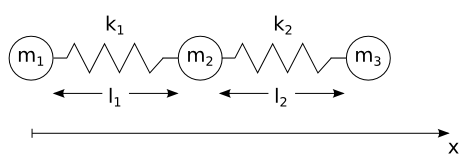
\includegraphics[width=0.6\textwidth]{images/3-masses-2-springs-linear.png}
  \caption{Diagram for 3 masses attached with springs representing the nuclei motion.}
  \label{fig:3-masses-2-springs}
\end{figure}
%
We will look only at the motion in the longitudinal direction so we attach a reference frame and call, as before, $x_i$ ($i=1,2,3$) the coordinate describing the position of $m_i$.
A lagrangian $L$ for this system is 
%
\begin{align}
L & = T-V\\ 
  & = \frac{1}{2}\sum_{i=1}^3 m_i \dot{x}_i^2 - \frac{1}{2}k_1(l_1-(x_2-x_1))^2+\frac{1}{2}k_2(l_2-(x_3-x_2))^2
\end{align}

It will be more convenient to change the $x_i$ coordinates to another set reflecting only the displacements from the equilibrium position.
That is, we define new coordinates $\eta_i$ such that $(x_1,x_2,x_3)=(\eta_1,l_1+\eta_2,l_1+l_2+\eta_3)$. 
In this coordinate system the lagrangian looks simpler
%
\begin{equation}
  L= \frac{1}{2}\sum_{i=1}^3 m_i \dot{\eta}_i^2-\frac{1}{2}k_1(\eta_1-\eta_2)^2+\frac{1}{2}k_2(\eta_2-\eta_3)^2
\end{equation}

The potential energy is a quadratic function of the $\eta_i$ displacements so we can write it in the general form $V=\frac{1}{2}\sum_{i,j}V_{ij}\eta_i\eta_j$ where $V_{ij}$ are the elements of the matrix defined as
%
\begin{equation}
  (V_{ij})=\left( \begin{array}{ccc} k_1 & -k_1 & 0 \\ -k_1 & k_1+k_2 & -k_2 \\ 0 & -k_2 & k_2 \end{array} \right)
\end{equation}
%
The dynamics of the system is determined by the Euler-Lagrange equations,
%
\begin{align}
  0 & = \frac{d}{dt}\frac{\partial L}{\partial \dot{\eta}_s}-\frac{\partial L}{\partial \eta_s} \label{eq:EulLag1} \\
    & = m_s \ddot{\eta}_s + \sum_i V_{is} \eta_i \label{eq:EulLag2}
\end{align}
%
for $s=1,2,3$. 
We can propose an oscillatory solution of the form $\eta_i=a_ie^{i\omega t}$, understanding that only the real part of this equations is physically significant.
Substituting this solution into the equations of motion (\ref{eq:EulLag2}), after removing the common exponential factor, gives
%
\begin{equation}
  0=\sum_i V_{is}a_i-\omega^2m_sa_s
\end{equation}
%
which can be arranged as a matrix
%
\begin{equation}
  \left( 
    \begin{array}{c} 
      0\\ 0\\ 0 
    \end{array}
  \right) = (V_{ij}) \left(
    \begin{array}{c}
      a_1 \\ a_2 \\ a_3 
    \end{array}
  \right) - \omega^2 \left(
    \begin{array}{ccc}
      m_1 & 0 & 0 \\ 0 & m_2 & 0 \\ 0 & 0 & m_3
    \end{array}\right) \left(
    \begin{array}{c} 
      a_1 \\ a_2 \\ a_3 
    \end{array}
  \right)
\end{equation}
%
Substituting the actual values for $(V_{ij})$:
%
\begin{equation}
  \left( 
    \begin{array}{c}
      0\\ 0\\ 0
    \end{array}
  \right) 
  = \left(
    \begin{array}{ccc}
      k_1-\omega^2m_1 & -k_1 & 0 \\ -k_1 & k_1+k_2-\omega^2m_2 & -k_2 \\ 0 & -k_2 & k_2-\omega^2m_3 
    \end{array}
  \right) 
  \left(
    \begin{array}{c}
      a_1 \\ a_2 \\ a_3 
    \end{array}
  \right)
\end{equation}
%
In order to have a non-trivial solution we require the determinant of that matrix to be zero
%
\begin{equation}
  \label{eq:det}
  \begin{split}
    0 = & (k_1-\omega^2m_1)(k_1+k_2-\omega^2m_2)(k_2-\omega^2m_3) \\
        & -k_1^2(k_2-\omega^2m_3)-k_2^2(k_1-\omega^2m_1)
  \end{split}
\end{equation}
%
which is a third order algebraic equation for $\omega^2$ with 3 solutions for $\omega$.
To simplify the calculation we take now into consideration the details of our problem, that is, we consider $m_1 = m_3 \equiv m_O$, $m_2 \equiv m_{Cu}$ and $k_1 = k_2 \equiv k$. 
With this considerations, (\ref{eq:det}) simplifies to
%
\begin{align}
  \label{eq:omegas}
  0 & = (k-\omega^2m_O)^2(2k-\omega^2m_{Cu})-2k^2(k-\omega^2m_O) \\
    & = (k-\omega^2m_O)[(k-\omega^2m_O)(2k-\omega^2m_{Cu})-2k^2]
\end{align}
%
from which we can observe one solution
%
\begin{equation}
  \omega^2= \frac{k}{m_O}
\end{equation}
%
corresponding to the symmetrical (Raman) vibrational mode, denoted by $\omega_{R}$ in \ref{eq:phonon-part}, since it doesn't depend on $m_{Cu}$.
The other two frequencies are obtained from the remaining factor in \ref{eq:omegas},
%
\begin{equation}
  \begin{split}
    0 & = (k-\omega^2m_O)(2k-\omega^2m_{Cu})-2k^2 \\
      & = 2k^2-k\omega^2m_{Cu}-2k\omega^2m_O+\omega^4m_Om_{Cu}-2k^2 \\
      & = \omega^2[\omega^2m_Om_{Cu}-k(m_{Cu}+2m_O)]
  \end{split}
\end{equation}
%
from here we obtain the uninteresting $\omega^2=0$ and
%
\begin{equation}
  \omega^2 = \frac{k(m_{Cu}+2m_O)}{m_Om_{Cu}}
\end{equation}

This is the frequency of the asymmetric (infrared) vibrational mode, denoted by $\omega_{ir}$ in (\ref{eq:phonon-part}).
Summarizing this part, we have found the dependence of the phonon frequencies $\omega_{ir}$ and $\omega_R$ with the atomic masses for the oxygen $m_O$ and copper $m_{Cu}$ atoms in the following way
%
\begin{equation}
  \label{eq:omegaR}
  \omega_{R}= \sqrt{\frac{k}{m_O}}
\end{equation}
%
\begin{equation}
  \label{eq:omegair}
  \omega_{ir} = \sqrt{\frac{k(m_{Cu}+2m_O)}{m_Om_{Cu}}}
\end{equation}
%
for some constant $k$.
From here we identify the reduced masses for each vibrational mode\footnote{We use $m_{Cu}=63.546u$, $m_{^{16}O}=15.995u$ and $m_{^{18}O}=17.999u$.}
%
\begin{equation}
  \label{eq:redMassR}
  m_R \equiv m_O \simeq 16.0\ u \simeq 2.6568 \times 10^{-26} kg
\end{equation}
%
\begin{equation}
  \label{eq:redMassIr}
  m_{ir} \equiv \frac{m_Om_{Cu}}{m_{Cu}+2m_O} \simeq 10.64\ u \simeq 1.7668 \times 10^{-26}kg
\end{equation}

From equations (\ref{eq:coupling-constants},\ref{eq:omegaR}, \ref{eq:omegair}) it can be seen that an oxygen isotope substitution $^{16}$O $\rightarrow$ $^{18}$O ammounts to a change in the frequencies  $(\omega_{ir}$, $\omega_R)$ and the coupling constants $(\lambda_{ir},\lambda_R)$.
Denoting as $\omega^{(16)}$ and $\omega^{(18)}$ the phonon frequencies for a cluster with $^{16}$O and $^{18}$O respectively, we can find the ratios
%
\begin{align}\label{eq:omega-isot}
  \omega^{(16)}_{ir}/\omega^{(18)}_{ir}
  & =\sqrt{\left(\frac{m_{^{18}O}}{m_{^{16}O}}\right)\left(\frac{m_{Cu}+2m_{^{16}O}}{m_{Cu}+2m_{^{18}O}}\right)} \\
  & \simeq 1.039 \\
  \omega^{(16)}_{R}/\omega^{(18)}_{R}
  & =\sqrt{\frac{m_{^{18}O}}{m_{^{16}O}}} \\
  & \simeq 1.061
\end{align}
%
Similarly, for the coupling constants $\lambda_{ir}$ and $\lambda_R$, from (\ref{eq:coupling-constants}), we can observe that
%
\begin{equation}
  \label{eq:lambda-ir-isot}
  \lambda_{ir}^{(16)}/\lambda_{ir}^{(18)}=\sqrt{\frac{m_{^{18}O}\omega_{ir}^{(18)}}{m_{^{16}O}\omega_{ir}^{(16)}}}\simeq 1.0407
\end{equation}
%
and equivalently for the Raman coupling constant
%
\begin{equation}
  \label{eq:lambda-Ram-isot}
  \lambda_R^{(16)} / \lambda_R^{(18)} \sqrt{\frac{m_{^{18}O}\omega_{R}^{(18)}}{m_{^{16}O}\omega_{R}^{(16)}}} \simeq 1.0299
\end{equation}

Summarizing, to model an isotopic substitution $^{16}$O$\rightarrow ^{18}$O we need to adjust the vibrational frequencies and coupling constants according to equations (\ref{eq:omega-isot}-\ref{eq:lambda-Ram-isot})

\section{Isotopic shifts}

As is customary in optical spectroscopies we will consider the relative isotopic shift $\Delta_i$ for an excited state $i$ as 
%
\begin{equation}
  \label{eq:isot-shift-def-exc}
  \Delta_i = \frac{\omega_i(^{16}O)- \omega_i(^{18}O)}{\omega_i(^{16}O)} \times 100
\end{equation}
%
where the energies $\omega_i$ are calculated relative to the corresponding ground state.
From this definition, using (\ref{eq:omegaR}, \ref{eq:omegair}), we can calculate the isotopic shift predicted by harmonic potentials for the Raman and infrared modes:
%
\begin{equation}
  \label{eq:isot-harm-R}
  \Delta_{R} = 1 - \frac{\omega_{R}(^{18}O)}{\omega_{R}(^{16}O)} \times 100 = 5.75\% 
\end{equation}
%
\begin{equation}
  \label{eq:isot-harm-ir}
  \Delta_{ir} = 1 - \frac{\omega_{ir}(^{18}O)}{\omega_{ir}(^{16}O)} \times 100 = 3.75\%
\end{equation}
%
Strong deviations from these values are indicative of a more complex behaviour.

% Discuss how anharmonic potentials give only positive isotopic shifts so negative values could mean polaronic behaviour.

For the ground state we define the energy isotopic shift $\Delta_g$ in a similar way but with the energies measured relative to the uncoupled system, that is, the system with $\lambda_{ir}=\lambda_R=0$,
%
\begin{equation}
  \label{eq:isot-shift-def-grd}
  \Delta_g = \frac{\Delta\omega_g(^{16}O)- \Delta\omega_g(^{18}O)}{\Delta \omega_g(^{16}O)} \times 100
\end{equation}
%
where $\Delta\omega_g \equiv \omega_g - \omega_g(\lambda_{ir}=0, \lambda_R=0)$. 
For the calculation of $\Delta_g$ it is essential to include the \textit{zero point energy} in the phononic part (\ref{eq:phonon-part}) which is usually not taken into account.

\section{Choice of parameters}
\label{sec:model-parameters}

To choose values for this model we take representative values guided from local-density approximations \cite{Pickett1989}. 
In particular Ref. \cite{DeWeert1989}, using a tight-binding model, reports a band energy of $E_0$ = 0.35 eV and a hopping parameter of $t=0.43-0.74$ eV, for Cu(1)-O(4) sites.
The on-site Coulomb repulsion in La$_2$CuO$_4$, $U$  is estimated to be in the range $4.0-10.5$ eV, \cite{Hybertsen1989}. 

The bare phonon frequency for the Raman vibrational mode is fixed to the value found experimentally in optical and inelastic neutron scattering experiments for YBa$_2$Cu$_3$O$_7$, namely $\omega_R = 500$ cm$^{-1}$ \cite{Thomsen1988,Cardona1988} and $\omega_{ir}$ is chosen such that the ratio $\omega_{ir}/\omega_R$ given by (\ref{eq:omegaR}-\ref{eq:omegair}) hold, which in this case gives $\omega_{ir} = 612.4$ cm$^{-1}$.

In order to consider the simplest possible model we make the further assumption of taking the on-site Coulomb repulsion in the copper and oxygen sites to be equal with no nearest neighbor Coulomb repulsion. 
We also use a single hopping parameter $t$ and ignore hopping between the two oxygen sites. 
Since only the coupling between the asymmetric mode and the charge motion leads to a measurable lattice distortion, with two Cu–O bond lengths, we only consider the effect of the variation in the electron–lattice coupling constant with the antisymmetric mode, $\lambda_{ir}$, and we set the electron-lattice coupling with the symmetric mode, $\lambda_R$ , as zero \cite{Salkola1995}. 
The inclusion of those considerations in the model, or other choices of parameters produce very similar results (e.g. \cite{Salkola1994, Salkola1995}).
The relevant value for the coupling $\lambda_{ir}$ is determined using equation \ref{eq:dvsuir}; it is chosen such that the ground state has a maximum probability density at a $u_{ir}$ that reproduces the observed lattice distortion of 0.13 \AA\ \cite{MustredeLeon1991}.
In this work we use the same parameters as in Refs. \cite{DeLeon1999, Leon2008, MirandaMena2007,Mena2006}, namely:

\begin{itemize*}
\item On-site Coulomb repulsion for O(4) and Cu(1) sites: $U=7$ eV
\item Nearest-neighbor hopping: $t=0.5$ eV
\item Band energy for O(4) and Cu(1) sites: $E_0=0.5$ eV
\item Bare phonon frequency for the Raman mode: $\omega_R=500$ cm$^{-1}$
\item Bare phonon frequency for the infrared mode: $\omega_{ir}=612.4$ cm$^{-1}$
\end{itemize*}

As previously stated, some variation in the parameter space has been explored without changes in the basic phenomenology. Table \ref{tab:parameters} shows the parameters for this model used in other publications\footnote{It seems that the reported values for the phonon frequencies in Refs. \cite{Salkola1994, Salkola1995} are erroneous since they show $\omega_R > \omega_{ir}$ and they are inconsistent from what can be observed, for example, in Fig. 1 of Ref. \cite{Salkola1994} at $\lambda_{ir}=0$.}.

\begin{table}[ht]
  \centering
  \begin{tabular}[h]{| l | c | c | c | c | c |}
    \hline
    Reference & $U$ (eV) & $\epsilon$ (eV) & $t$ (eV) & $\omega_{ir}$ (cm$^{-1}$) & $\omega_R$(cm$^{-1)}$ \\
    \hline
    \cite{MustredeLeon1992} & 7.0 & 0.5 & 0.5 & 600 & 500 \\ 
    \cite{Salkola1994, Salkola1995} & 4.44 & 0.307 & 0.634 & 477.7 & 576  \\
    \cite{DeLeon1999, Leon2008, MirandaMena2007,Mena2006} & 7.0 & 0.5 & 0.5 & 612.4 & 500 \\ 
    \cite{MustredeLeon2000} & 4.44 & 0.307 & 0.634 & 600 & 500 \\
    \hline
  \end{tabular}
  \caption{Parameters for the model hamiltonian (\ref{eq:full-hamiltonian}) used in other publications.}
  \label{tab:parameters}
\end{table}
